\documentclass[tikz]{tmr}

\title{Two Monoids for Approximating NP-Complete Problems}
\author{Mike Izbicki\email{mike@izbicki.me}}

\usepackage{rotating}
\usepackage{listings}
\lstloadlanguages{Haskell}
\lstnewenvironment{spec}
    {\lstset{}%
      \csname lst@SetFirstLabel\endcsname}
    {\csname lst@SaveFirstLabel\endcsname}
    \lstset{
      basicstyle=\small\ttfamily,
      xleftmargin=\parindent,
      xleftmargin=\parindent,
      flexiblecolumns=false,
      keepspaces=true,
      basewidth={0.5em,0.45em},
      literate={+}{{$+$}}1 {/}{{$/$}}1 {*}{{$*$}}1 {=}{{$=$}}1
               {>}{{$>$}}1 {<}{{$<$}}1 {\\}{{$\lambda$}}1
               {\\\\}{{\char`\\\char`\\}}1
               {->}{{$\rightarrow$}}2 {>=}{{$\geq$}}2 {<-}{{$\leftarrow$}}2
               {<=}{{$\leq$}}2 {=>}{{$\Rightarrow$}}2 
%                {\ .}{{$\circ$}}2 {\ .\ }{{$\circ$}}2
               {>>}{{>>}}2 {>>=}{{>>=}}2
               {|}{{$\mid$}}1               
               {<>}{{$\diamond$}}1          
               {++}{{$\+$}}1                
               {mempty}{{$\epsilon$}}1               
    }
\lstnewenvironment{code}
    {\lstset{}%
      \csname lst@SetFirstLabel\endcsname}
    {\csname lst@SaveFirstLabel\endcsname}
    \lstset{
      numbers=left,
%       stepnumber=5,    
      firstnumber=1,
      numberfirstline=true,
      basicstyle=\small\ttfamily,
      xleftmargin=\parindent,
      xleftmargin=\parindent,
      flexiblecolumns=false,
      keepspaces=true,
      basewidth={0.5em,0.45em},
      literate={+}{{$+$}}1 {/}{{$/$}}1 {*}{{$*$}}1 {=}{{$=$}}1
               {>}{{$>$}}1 {<}{{$<$}}1 {\\}{{$\lambda$}}1
               {\\\\}{{\char`\\\char`\\}}1
               {->}{{$\rightarrow$}}2 {>=}{{$\geq$}}2 {<-}{{$\leftarrow$}}2
               {<=}{{$\leq$}}2 {=>}{{$\Rightarrow$}}2 
%                {\ .}{{$\circ$}}2 {\ .\ }{{$\circ$}}2
               {>>}{{>>}}2 {>>=}{{>>=}}2
               {|}{{$\mid$}}1               
               {<>}{{$\diamond$}}1          
               {++}{{$\+$}}1                
               {mempty}{{$\epsilon$}}1               
    }
\newcommand{\prob}[1]{{\sc {#1}}}
\newcommand{\np}{{\ensuremath{\mathbb{NP}}}}

\newcommand\doubleplus{+\kern-1.3ex+\kern0.8ex}
\newcommand\+{\mdoubleplus}
\newcommand\mdoubleplus{\ensuremath{\mathbin{+\mkern-10mu+}}}


\begin{document}

\begin{introduction}
As a TA I was confronted with a real life instance of the NP-complete Scheduling problem.
To solve the problem, I turned to the classic LPTF approximation algorithm.
In this article, we'll see that because LPTF is a monoid homomorphism, we can implement it using the HomTrainer  type class.
This gives us parallel and iterative versions of LPTF ``for free.''
What's more, LPTF is a particularly illustrative instance of HomTrainer for three reasons.
First, the monoid operation for Scheduling takes non-constant time, and the HomTrainer class makes reasoning about this run time straightforward.
Second, the monoid uses lazy semantics to improve performance.  
Finally, it demonstrates the versatility of the HomTrainer to domains outside of machine learning.
\end{introduction}

\section{Discovering The Problem}
I enjoy teaching.  
It's really fun helping my intro to C++ students struggle through pointer arithmetic.  
(I doubt the students feel the same way after spending five hours tracking down a segfault!)
%(It's only fun because \emph{I} am not the one spending hours tracking down the segfaults!)
% Ah, the joys of segfaults... 
%(to be young and segfaulting...)
But teaching is even better when it causes you to stumble onto an interesting research question.  
Oddly enough, I found a cool Haskell problem while TAing a class in C++ last quarter.

The professor wanted to assign a group project, and I had to pick the groups.
The only requirement was that the groups should be as fair as possible.
%He didn't want to let students pick their own groups because he wanted the groups to be as fair as possible.
In other words, the best and worst students should be evenly distributed throughout all the groups.
Because of this requirement, the students couldn't pick their own groups.

``Aha!'' I said to myself, ``This sounds like the optimization version of the NP-complete Multiprocessor Scheduling problem.''  

We'll just call it \prob{Scheduling} for short.  
In the \prob{Scheduling} problem, we are given $k$ processors and $n$ tasks.
Each task $t_i$ has some time it will take to complete it, called $\lvert t_i \rvert$.
The goal is to assign the tasks to processors in a way that will minimize the total amount of time it takes to complete the tasks.
This is shown graphically in Figure \ref{fig:scheduling}.

\begin{figure}[H]
\centering
\caption{The \prob{Scheduling} problem}
\label{fig:scheduling}
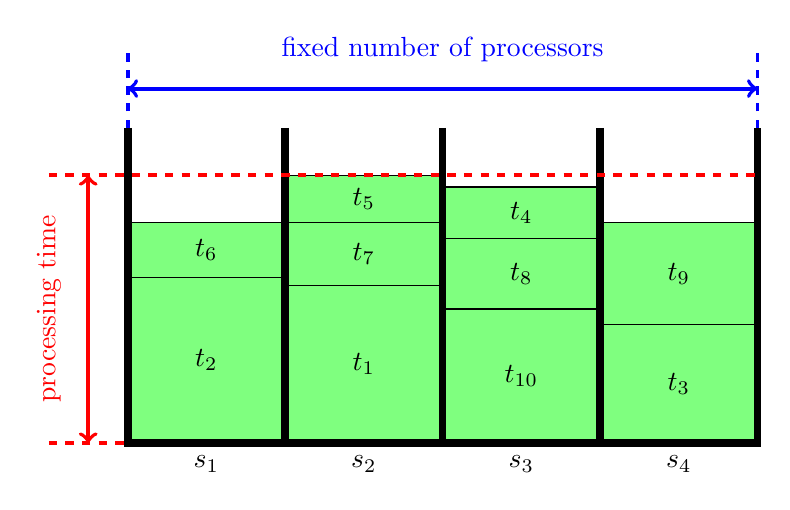
\begin{tikzpicture}
\definecolor{hlearn_bgbox}{RGB}{127,255,127}
\node[shape=rectangle,draw,fill=hlearn_bgbox,minimum width=2cm,minimum height=2.1cm] at (3,1.05) { $t_{2}$ };
\node[shape=rectangle,draw,fill=hlearn_bgbox,minimum width=2cm,minimum height=0.7cm] at (3,2.45) { $t_{6}$ };
\node[shape=rectangle,draw,fill=hlearn_bgbox,minimum width=2cm,minimum height=2.0cm] at (5,1.0) { $t_{1}$ };
\node[shape=rectangle,draw,fill=hlearn_bgbox,minimum width=2cm,minimum height=0.8cm] at (5,2.4) { $t_{7}$ };
\node[shape=rectangle,draw,fill=hlearn_bgbox,minimum width=2cm,minimum height=0.6cm] at (5,3.0999999999999996) { $t_{5}$ };
\node[shape=rectangle,draw,fill=hlearn_bgbox,minimum width=2cm,minimum height=1.7cm] at (7,0.85) { $t_{10}$ };
\node[shape=rectangle,draw,fill=hlearn_bgbox,minimum width=2cm,minimum height=0.9cm] at (7,2.15) { $t_{8}$ };
\node[shape=rectangle,draw,fill=hlearn_bgbox,minimum width=2cm,minimum height=0.65cm] at (7,2.9250000000000003) { $t_{4}$ };
\node[shape=rectangle,draw,fill=hlearn_bgbox,minimum width=2cm,minimum height=1.5cm] at (9,0.75) { $t_{3}$ };
\node[shape=rectangle,draw,fill=hlearn_bgbox,minimum width=2cm,minimum height=1.3cm] at (9,2.15) { $t_{9}$ };
\draw[line width=0.1cm] (2,4) to (2,0) to node[below] {$s_{1}$} (2+2,0) to (2+2,4);
\draw[line width=0.1cm] (4,4) to (4,0) to node[below] {$s_{2}$} (4+2,0) to (4+2,4);
\draw[line width=0.1cm] (6,4) to (6,0) to node[below] {$s_{3}$} (6+2,0) to (6+2,4);
\draw[line width=0.1cm] (8,4) to (8,0) to node[below] {$s_{4}$} (8+2,0) to (8+2,4);

\draw[dashed,color=red,line width=0.05cm] (1,3.4) to (10,3.4);
\draw[dashed,color=red,line width=0.05cm] (1,0) to (2,0);
\draw[<->,color=red,line width=0.05cm] (1.5,3.4) to  (1.5,0);
\node[color=red] at (1,1.7) {\rotatebox{90}{processing time}};
\draw[dashed,color=blue,line width=0.05cm] (2,4) to (2,5);
\draw[dashed,color=blue,line width=0.05cm] (10,4) to (10,5);
\draw[<->,color=blue,line width = 0.05cm] (2,4.5) to (10,4.5);
\node[color=blue] at (6,5) {fixed number of processors};
\end{tikzpicture}
\vspace{0.1in}
\end{figure}

So how is this like the problem my professor gave me?
Well, we can think of the number of groups as the number of processors, each task is a student, and the amount of time it takes to complete a task is a measure of how good a student is.
Then, the problem is to find a way to divvy up the students so that the total goodness for each group is as close as possible.

\prob{Scheduling} is closely related to another \np-complete problem called \prob{Bin Packing}.
In this problem, instead of fixing the number of bins and minimizing the amount in the bins, we fix the amount each bin can store and minimize the total number of bins used.
See Figure \ref{fig:binpacking}.

Both \prob{Scheduling} and \prob{Bin Packing} have a number of important applications.

\begin{figure}[H]
\caption{The \prob{Bin Packing} problem}
\label{fig:binpacking}
\centering
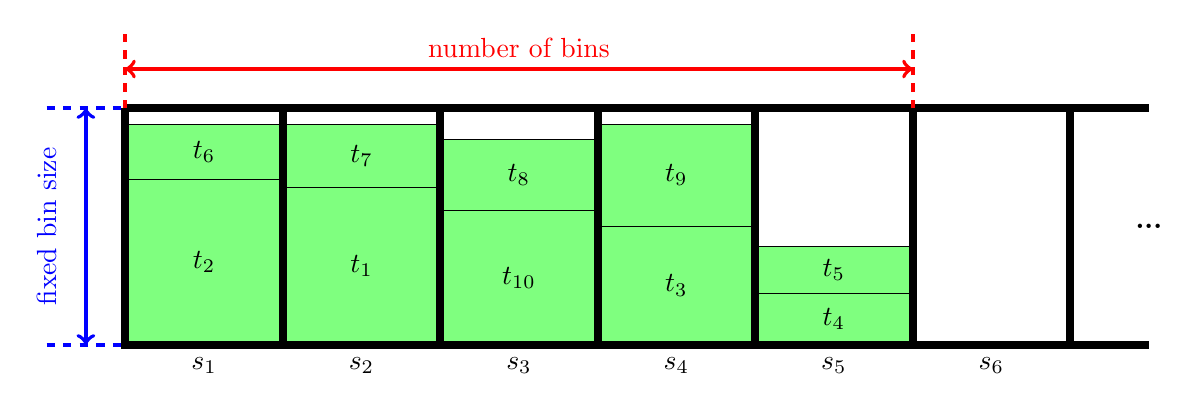
\begin{tikzpicture}
\definecolor{hlearn_bgbox}{RGB}{127,255,127}
\node[shape=rectangle,draw,fill=hlearn_bgbox,minimum width=2cm,minimum height=2.1cm] at (3,1.05) { $t_{2}$ };
\node[shape=rectangle,draw,fill=hlearn_bgbox,minimum width=2cm,minimum height=0.7cm] at (3,2.45) { $t_{6}$ };
\node[shape=rectangle,draw,fill=hlearn_bgbox,minimum width=2cm,minimum height=2.0cm] at (5,1.0) { $t_{1}$ };
\node[shape=rectangle,draw,fill=hlearn_bgbox,minimum width=2cm,minimum height=0.8cm] at (5,2.4) { $t_{7}$ };
\node[shape=rectangle,draw,fill=hlearn_bgbox,minimum width=2cm,minimum height=1.7cm] at (7,0.85) { $t_{10}$ };
\node[shape=rectangle,draw,fill=hlearn_bgbox,minimum width=2cm,minimum height=0.9cm] at (7,2.15) { $t_{8}$ };
\node[shape=rectangle,draw,fill=hlearn_bgbox,minimum width=2cm,minimum height=1.5cm] at (9,0.75) { $t_{3}$ };
\node[shape=rectangle,draw,fill=hlearn_bgbox,minimum width=2cm,minimum height=1.3cm] at (9,2.15) { $t_{9}$ };
\node[shape=rectangle,draw,fill=hlearn_bgbox,minimum width=2cm,minimum height=0.65cm] at (11,0.325) { $t_{4}$ };
\node[shape=rectangle,draw,fill=hlearn_bgbox,minimum width=2cm,minimum height=0.6cm] at (11,0.95) { $t_{5}$ };
\draw[line width=0.1cm] (2,3.0) to (2,0) to node[below] {$s_{1}$} (2+2,0) to (2+2,3.0);
\draw[line width=0.1cm] (4,3.0) to (4,0) to node[below] {$s_{2}$} (4+2,0) to (4+2,3.0);
\draw[line width=0.1cm] (6,3.0) to (6,0) to node[below] {$s_{3}$} (6+2,0) to (6+2,3.0);
\draw[line width=0.1cm] (8,3.0) to (8,0) to node[below] {$s_{4}$} (8+2,0) to (8+2,3.0);
\draw[line width=0.1cm] (10,3.0) to (10,0) to node[below] {$s_{5}$} (10+2,0) to (10+2,3.0);
\draw[line width=0.1cm] (12,3.0) to (12,0) to node[below] {$s_{6}$} (12+2,0) to (12+2,3.0);
% \draw[line width=0.1cm] (14,3.0) to (14,0) to node[below] {$s_{5}$} (14+2,0) to (14+2,3.0);
% \draw[line width=0.1cm] (16,3.0) to (16,0) to node[below] {$s_{5}$} (16+2,0) to (16+2,3.0);
\draw[line width=0.1cm] (2,3.0) to (15,3.0);
\draw[line width=0.1cm] (2,0) to (15,0);
\draw[dashed,color=red,line width=0.05cm] (2,3) to (2,4);
\draw[dashed,color=red,line width=0.05cm] (12,3) to (12,4);
\draw[<->,line width=0.05cm,color=red] (2,3.5) to node[above] {number of bins} (12,3.5);
\draw[<->,line width=0.05cm,color=blue] (1.5,0) to (1.5,3);
\draw[dashed,color=blue,line width=0.05cm] (1,0) to (2,0);
\draw[dashed,color=blue,line width=0.05cm] (1,3) to (2,3);
\node[color=blue] at (1,1.5) {\rotatebox{90}{fixed bin size}};
\node at (15,1.5) {\textbf{...}};
\end{tikzpicture}
\end{figure}

Since \prob{Scheduling} is \np-complete, finding an exact solution takes exponential time.  
I had no chance of creating an optimal grouping for my professor---the class had 100 students, and $2^{100}$ is a BIG number!
So I turned to approximation algorithms.
These algorithms give us solutions that are guaranteed to be within a certain factor of optimal.
One popular approximation algorithm for \prob{Scheduling} is called Longest Processing Time First (LPTF).
LPTF always returns a schedule whose time is guaranteed to be less than $4/3$ times the optimal.
This is often written as:
$$
LPTF = {4\over3} OPT
$$
And we call LPTF a $4\over 3$-approximation.
By making this small sacrifice in accuracy, we get an algorithm that runs in time $\Theta(n\log n)$ instead of $\Theta(2^n)$.

\section{The \prob{Scheduling} HomTrainer}



I wanted to implement LPTF using the HomTrainer type class because the compiler automatically derives online and parallel algorithms for all instances of HomTrainer.
To get this benefit, our algorithm must be a \emph{monoid homomorphism} from the \emph{free monoid}.
This sounds a lot scarier than it actually is.

\begin{figure}[H]
\caption{Basic requirements of the HomTrainer type class}
\centering
\tikzstyle{blackbox}=[shape=rectangle, draw, fill=black, text=white, minimum width=0.8in]
\begin{tikzpicture}%[node distance=2.5in, auto, >=stealth]
\node[blackbox] (dataset) [minimum height=0.3in] {\textbf{data set}};
\node[blackbox] (model)   [minimum height=0.3in, node distance=2in,right of = dataset] {\textbf{model}};
\node[blackbox] (answer)  [minimum height=0.3in, node distance=2in,right of = model] {\textbf{answer}};
\draw[->,ultra thick] (dataset) to node[above] {train} (model);
\draw[->,ultra thick] (model) to node[above] {question} (answer);

\node (l1) [color=blue] at (-0.1,-1.3) {free monoid};
\node (l2) [color=blue] at (2.5,1.5) {homomorphism};
\node (l3) [color=blue] at (5.5,-1.3) {monoid};

\draw[->,color=blue,ultra thick] (l1) to (dataset);
\draw[->,color=blue,ultra thick] (l2) to (2.5,0.5);
\draw[->,color=blue,ultra thick] (l3) to (model);
\end{tikzpicture}
\vspace{0.15in}
\end{figure}

In Haskell, the Monoid type class is defined as:
% \begin{figure}
% \caption{Monoid type class}
\begin{spec}
class Monoid m where
    mempty  :: m
    mappend :: m -> m -> m
\end{spec}
% \end{figure}
and all instances of Monoid obey the law that:
$$
\epsilon \diamond m = m\diamond \epsilon = m
$$

Lists are one of the simplest examples of monoids.

\begin{spec}
instance Monoid [a] where
    mempty = []
    mappend = ++
\end{spec}

Lists are also one example of free monoids.
Basically, any container that is a monoid is a free monoid.
For example, vectors and sets are also free monoids.

When we say that our algorithm must be a monoid homomorphism from a free monoid, we mean that it has the type:
\begin{spec}
train :: [Datapoint] -> Scheduling
\end{spec}
And it obeys the law that for all \lstinline{xs} and \lstinline{ys} of type \lstinline{[Datapoint]}:
\begin{spec}
train (xs ++ ys) = (train xs) <> (train ys)
\end{spec}

In picture form, what we needed of our LPTF algorithm is shown in Figure \ref{fig:LPTF-monoid}.

\begin{figure}[H]
\caption{The Monoid operation illustrated}
\label{fig:LPTF-monoid}
\centering
\begin{tikzpicture}

\node at (-2in,4) {
    \resizebox{1.75in}{!}{
    \begin{tikzpicture}
    \definecolor{hlearn_bgbox}{RGB}{127,255,127}
    \definecolor{hlearn_bgboxB}{RGB}{191,191,255}
    \node[shape=rectangle,draw,fill=hlearn_bgbox,minimum width=2cm,minimum height=2.1cm]   at (1,1.05) { $t_{a,1}$ };
    \node[shape=rectangle,draw,fill=hlearn_bgbox,minimum width=2cm,minimum height=2.7cm]   at (3,1.35) { $t_{a,2}$ };
    \node[shape=rectangle,draw,fill=hlearn_bgbox,minimum width=2cm,minimum height=3.1cm]   at (5,1.55) { $t_{a,3}$ };;
    \node[shape=rectangle,draw,fill=hlearn_bgbox,minimum width=2cm,minimum height=1.7cm]   at (7,0.85) { $t_{a,4}$ };
    \node[shape=rectangle,draw,fill=hlearn_bgbox,minimum width=2cm,minimum height=1.6cm]   at (9,0.8) { $t_{a,5}$ };
    \node[shape=rectangle,draw,fill=hlearn_bgbox,minimum width=2cm,minimum height=0.6cm]   at (11,0.3) { $t_{a,6}$ };
    \end{tikzpicture}
    }};

\node at (-2in,0) {
    \resizebox{1.5in}{!}{
    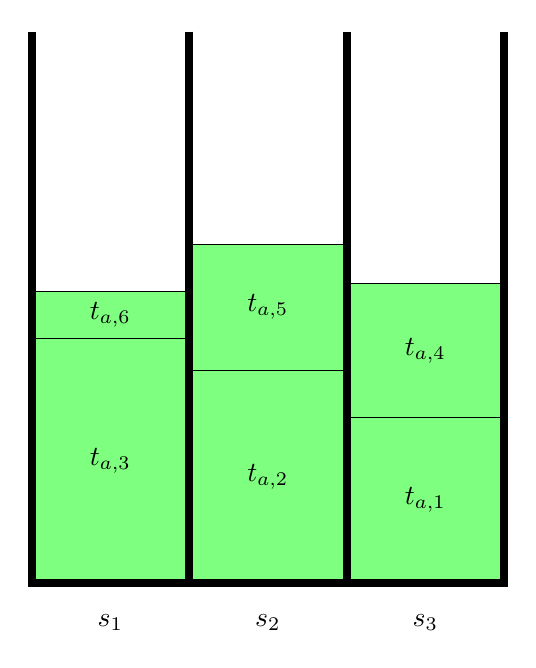
\begin{tikzpicture}
    \definecolor{hlearn_bgbox}{RGB}{127,255,127}
    \node[shape=rectangle,draw,fill=hlearn_bgbox,minimum width=2cm,minimum height=3.1cm] at (3,1.55) { $t_{a,3}$ };
    \node[shape=rectangle,draw,fill=hlearn_bgbox,minimum width=2cm,minimum height=0.6cm] at (3,3.4) { $t_{a,6}$ };
    \node[shape=rectangle,draw,fill=hlearn_bgbox,minimum width=2cm,minimum height=2.7cm] at (5,1.35) { $t_{a,2}$ };
    \node[shape=rectangle,draw,fill=hlearn_bgbox,minimum width=2cm,minimum height=1.6cm] at (5,3.5) { $t_{a,5}$ };
    \node[shape=rectangle,draw,fill=hlearn_bgbox,minimum width=2cm,minimum height=2.1cm] at (7,1.05) { $t_{a,1}$ };
    \node[shape=rectangle,draw,fill=hlearn_bgbox,minimum width=2cm,minimum height=1.7cm] at (7,2.95) { $t_{a,4}$ };
    \draw[line width=0.1cm] (2,7.0) to (2,0) to (2+2,0) to (2+2,7.0);
    \draw[line width=0.1cm] (4,7.0) to (4,0) to (4+2,0) to (4+2,7.0);
    \draw[line width=0.1cm] (6,7.0) to (6,0) to (6+2,0) to (6+2,7.0);
    \node at (3,-0.5) {$s_{1}$};
    \node at (5,-0.5) {$s_{2}$};
    \node at (7,-0.5) {$s_{3}$};
    \end{tikzpicture}
    }};

\node at (0,4) {
    \resizebox{1.75in}{!}{
    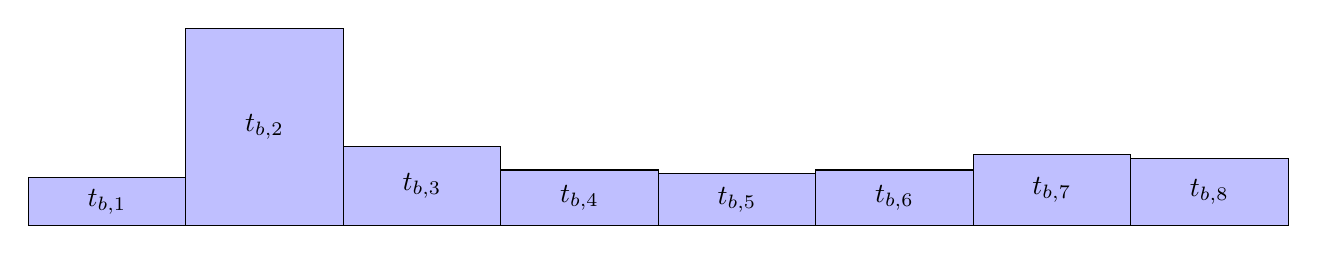
\begin{tikzpicture}
    \definecolor{hlearn_bgbox}{RGB}{127,255,127}
    \definecolor{hlearn_bgboxB}{RGB}{191,191,255}
    \node[shape=rectangle,draw,fill=hlearn_bgboxB,minimum width=2cm,minimum height=0.6cm]  at (1,0.3) { $t_{b,1}$ };
    \node[shape=rectangle,draw,fill=hlearn_bgboxB,minimum width=2cm,minimum height=2.5cm]  at (3,1.25) { $t_{b,2}$ };
    \node[shape=rectangle,draw,fill=hlearn_bgboxB,minimum width=2cm,minimum height=1.0cm]  at (5,0.5) { $t_{b,3}$ };
    \node[shape=rectangle,draw,fill=hlearn_bgboxB,minimum width=2cm,minimum height=0.7cm]  at (7,0.35) { $t_{b,4}$ };
    \node[shape=rectangle,draw,fill=hlearn_bgboxB,minimum width=2cm,minimum height=0.65cm] at (9,0.325) { $t_{b,5}$ };
    \node[shape=rectangle,draw,fill=hlearn_bgboxB,minimum width=2cm,minimum height=0.7cm]  at (11,0.35) { $t_{b,6}$ };
    \node[shape=rectangle,draw,fill=hlearn_bgboxB,minimum width=2cm,minimum height=0.9cm]  at (13,0.45) { $t_{b,7}$ };
    \node[shape=rectangle,draw,fill=hlearn_bgboxB,minimum width=2cm,minimum height=0.85cm] at (15,0.425) { $t_{b,8}$ };
    \end{tikzpicture}
    }};

\node at (0,0) {
    \resizebox{1.5in}{!}{
    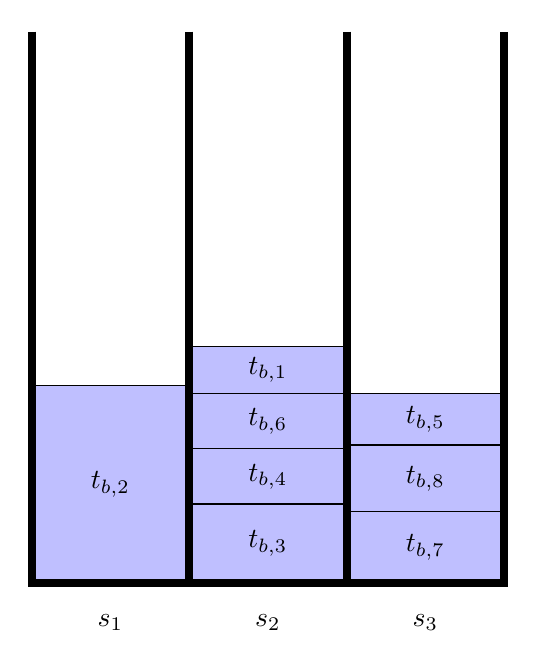
\begin{tikzpicture}
    \definecolor{hlearn_bgboxB}{RGB}{191,191,255}
    \node[shape=rectangle,draw,fill=hlearn_bgboxB,minimum width=2cm,minimum height=2.5cm] at (3,1.25) { $t_{b,2}$ };
    \node[shape=rectangle,draw,fill=hlearn_bgboxB,minimum width=2cm,minimum height=1.0cm] at (5,0.5) { $t_{b,3}$ };
    \node[shape=rectangle,draw,fill=hlearn_bgboxB,minimum width=2cm,minimum height=0.7cm] at (5,1.35) { $t_{b,4}$ };
    \node[shape=rectangle,draw,fill=hlearn_bgboxB,minimum width=2cm,minimum height=0.7cm] at (5,2.05) { $t_{b,6}$ };
    \node[shape=rectangle,draw,fill=hlearn_bgboxB,minimum width=2cm,minimum height=0.6cm] at (5,2.6999999999999997) { $t_{b,1}$ };
    \node[shape=rectangle,draw,fill=hlearn_bgboxB,minimum width=2cm,minimum height=0.9cm] at (7,0.45) { $t_{b,7}$ };
    \node[shape=rectangle,draw,fill=hlearn_bgboxB,minimum width=2cm,minimum height=0.85cm] at (7,1.325) { $t_{b,8}$ };
    \node[shape=rectangle,draw,fill=hlearn_bgboxB,minimum width=2cm,minimum height=0.65cm] at (7,2.075) { $t_{b,5}$ };
    \draw[line width=0.1cm] (2,7.0) to (2,0) to (2+2,0) to (2+2,7.0);
    \draw[line width=0.1cm] (4,7.0) to (4,0) to (4+2,0) to (4+2,7.0);
    \draw[line width=0.1cm] (6,7.0) to (6,0) to (6+2,0) to (6+2,7.0);
    \node at (3,-0.5) {$s_{1}$};
    \node at (5,-0.5) {$s_{2}$};
    \node at (7,-0.5) {$s_{3}$};
    \end{tikzpicture}
    }};

\node at (2in,4) {
    \resizebox{1.75in}{!}{
    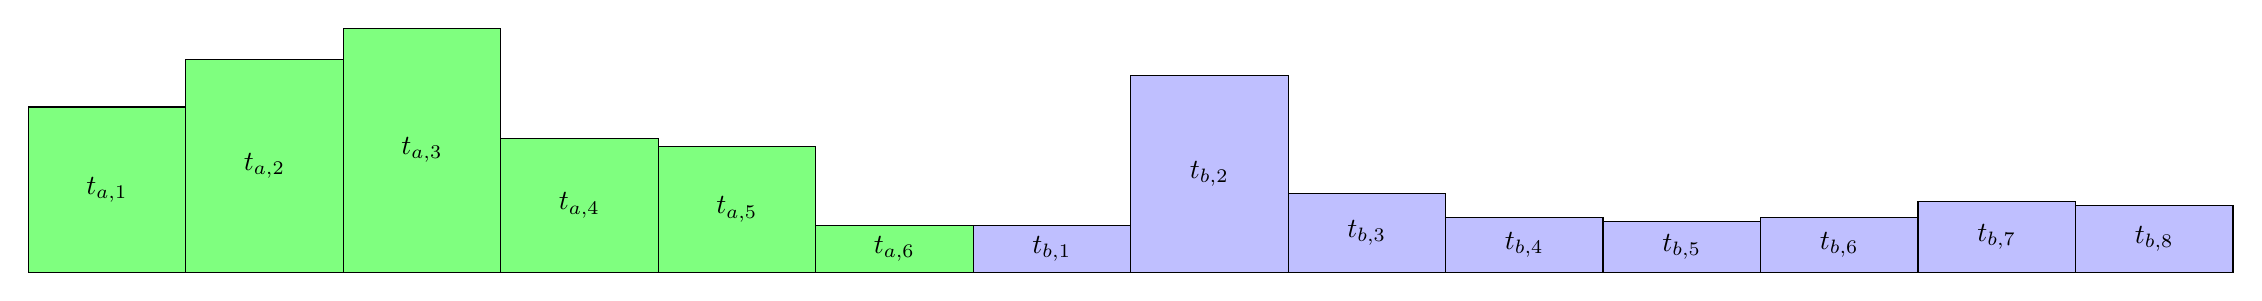
\begin{tikzpicture}
    \definecolor{hlearn_bgbox}{RGB}{127,255,127}
    \definecolor{hlearn_bgboxB}{RGB}{191,191,255}
    \node[shape=rectangle,draw,fill=hlearn_bgbox,minimum width=2cm,minimum height=2.1cm]   at (1,1.05) { $t_{a,1}$ };
    \node[shape=rectangle,draw,fill=hlearn_bgbox,minimum width=2cm,minimum height=2.7cm]   at (3,1.35) { $t_{a,2}$ };
    \node[shape=rectangle,draw,fill=hlearn_bgbox,minimum width=2cm,minimum height=3.1cm]   at (5,1.55) { $t_{a,3}$ };;
    \node[shape=rectangle,draw,fill=hlearn_bgbox,minimum width=2cm,minimum height=1.7cm]   at (7,0.85) { $t_{a,4}$ };
    \node[shape=rectangle,draw,fill=hlearn_bgbox,minimum width=2cm,minimum height=1.6cm]   at (9,0.8) { $t_{a,5}$ };
    \node[shape=rectangle,draw,fill=hlearn_bgbox,minimum width=2cm,minimum height=0.6cm]   at (11,0.3) { $t_{a,6}$ };
    \node[shape=rectangle,draw,fill=hlearn_bgboxB,minimum width=2cm,minimum height=0.6cm]  at (13,0.3) { $t_{b,1}$ };
    \node[shape=rectangle,draw,fill=hlearn_bgboxB,minimum width=2cm,minimum height=2.5cm]  at (15,1.25) { $t_{b,2}$ };
    \node[shape=rectangle,draw,fill=hlearn_bgboxB,minimum width=2cm,minimum height=1.0cm]  at (17,0.5) { $t_{b,3}$ };
    \node[shape=rectangle,draw,fill=hlearn_bgboxB,minimum width=2cm,minimum height=0.7cm]  at (19,0.35) { $t_{b,4}$ };
    \node[shape=rectangle,draw,fill=hlearn_bgboxB,minimum width=2cm,minimum height=0.65cm] at (21,0.325) { $t_{b,5}$ };
    \node[shape=rectangle,draw,fill=hlearn_bgboxB,minimum width=2cm,minimum height=0.7cm]  at (23,0.35) { $t_{b,6}$ };
    \node[shape=rectangle,draw,fill=hlearn_bgboxB,minimum width=2cm,minimum height=0.9cm]  at (25,0.45) { $t_{b,7}$ };
    \node[shape=rectangle,draw,fill=hlearn_bgboxB,minimum width=2cm,minimum height=0.85cm] at (27,0.425) { $t_{b,8}$ };
    \end{tikzpicture}
    }};

\node at (2in,0) {
    \resizebox{1.5in}{!}{
    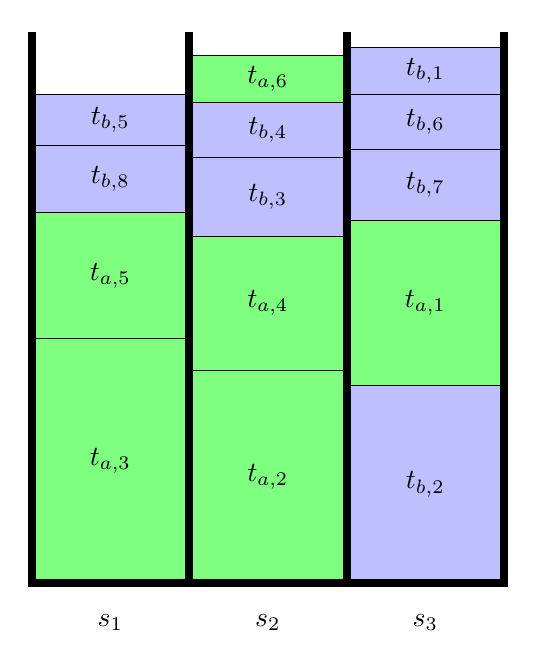
\begin{tikzpicture}
    \definecolor{hlearn_bgbox}{RGB}{127,255,127}
    \definecolor{hlearn_bgboxB}{RGB}{191,191,255}
    \node[shape=rectangle,draw,fill=hlearn_bgbox,minimum width=2cm,minimum height=3.1cm] at (3,1.55) { $t_{a,3}$ };
    \node[shape=rectangle,draw,fill=hlearn_bgbox,minimum width=2cm,minimum height=1.6cm] at (3,3.9000000000000004) { $t_{a,5}$ };
    \node[shape=rectangle,draw,fill=hlearn_bgboxB,minimum width=2cm,minimum height=0.85cm] at (3,5.125) { $t_{b,8}$ };
    \node[shape=rectangle,draw,fill=hlearn_bgboxB,minimum width=2cm,minimum height=0.65cm] at (3,5.875) { $t_{b,5}$ };
    \node[shape=rectangle,draw,fill=hlearn_bgbox,minimum width=2cm,minimum height=2.7cm] at (5,1.35) { $t_{a,2}$ };
    \node[shape=rectangle,draw,fill=hlearn_bgbox,minimum width=2cm,minimum height=1.7cm] at (5,3.5500000000000003) { $t_{a,4}$ };
    \node[shape=rectangle,draw,fill=hlearn_bgboxB,minimum width=2cm,minimum height=1.0cm] at (5,4.9) { $t_{b,3}$ };
    \node[shape=rectangle,draw,fill=hlearn_bgboxB,minimum width=2cm,minimum height=0.7cm] at (5,5.75) { $t_{b,4}$ };
    \node[shape=rectangle,draw,fill=hlearn_bgbox,minimum width=2cm,minimum height=0.6cm] at (5,6.4) { $t_{a,6}$ };
    \node[shape=rectangle,draw,fill=hlearn_bgboxB,minimum width=2cm,minimum height=2.5cm] at (7,1.25) { $t_{b,2}$ };
    \node[shape=rectangle,draw,fill=hlearn_bgbox,minimum width=2cm,minimum height=2.1cm] at (7,3.55) { $t_{a,1}$ };
    \node[shape=rectangle,draw,fill=hlearn_bgboxB,minimum width=2cm,minimum height=0.9cm] at (7,5.05) { $t_{b,7}$ };
    \node[shape=rectangle,draw,fill=hlearn_bgboxB,minimum width=2cm,minimum height=0.7cm] at (7,5.85) { $t_{b,6}$ };
    \node[shape=rectangle,draw,fill=hlearn_bgboxB,minimum width=2cm,minimum height=0.6cm] at (7,6.5) { $t_{b,1}$ };
    \draw[line width=0.1cm] (2,7.0) to (2,0) to (2+2,0) to (2+2,7.0);
    \draw[line width=0.1cm] (4,7.0) to (4,0) to (4+2,0) to (4+2,7.0);
    \draw[line width=0.1cm] (6,7.0) to (6,0) to (6+2,0) to (6+2,7.0);
    \node at (3,-0.5) {$s_{1}$};
    \node at (5,-0.5) {$s_{2}$};
    \node at (7,-0.5) {$s_{3}$};
    \end{tikzpicture}
    }};

\node at (-1in,0) {$\diamond$};
\node at (1in,0) {$=$};
\node at (-1in,4) {$\+$};
\node at (1in,4) {$=$};

\node at (-3in,4) {\rotatebox{90}{data sets}};
\node at (-3in,0) {\rotatebox{90}{model}};

\draw[dotted] (-3in,3) to (3in,3);

\draw[->,line width=0.05cm,color=orange] (-2in,3.3) to (-2in,2.5);

\end{tikzpicture}
\end{figure}


\section {Using the Partition Monoid}

First, this document is a literate Haskell file.
In order to run it, you'll need to download the latest HLearn-datastructures library:

\begin{verbatim}
 > cabal install hlearn-datastructures-1.0.0
\end{verbatim}

Let's ask GHCI about the kind of our scheduling type:

\begin{lstlisting}
ghci> :kind Scheduling
Scheduling :: Nat -> * -> *
\end{lstlisting}

This means that Scheduling takes two parameters.  
The first is of kind Nat, which means it is a type level natural number.
This is the number of processors that will be in our schedule.
The second is of kind * and represents the type for the tasks that we are going to schedule.
These tasks can be of any type at all.
But, if we are going to use our HomTrainer instance, then we have to satisfy some constraints.

\begin{lstlisting}
ghci> :info Scheduling
...
instance (Norm a) => HomTrainer (Scheduling n a) where
...
\end{lstlisting}

In particular, whatever type are tasks are, they must be an instance of Norm.
What does that mean?
In mathematics, a type has a norm if it has a ``size'' of some sort.
The most common norm is the Euclidean norm on vector spaces.
This is given by the pythagorean theorem:

In HLearn, anything with a size implements the Norm type class, which is defined as:
\begin{lstlisting}
class (HasRing m, Ord (Ring m)) => Norm m where
    magnitude :: m -> Ring m

class (Num (Ring m)) => HasRing m where
    type Ring m
\end{lstlisting}

% Our example begins, as always, with some language extensions and imports.
% 
% \begin{spec}
% {-# LANGUAGE TypeFamilies #-}
% {-# LANGUAGE DataKinds #-}
% 
% import Data.Csv
% import System.IO
% import qualified Data.ByteString.Lazy.Char8  as BS
% import qualified Data.Vector  as V
% 
% import HLearn.Algebra
% import HLearn.NPHard.Scheduling
% \end{spec}
% 
% Now we're ready to start our problem.  
% We begin by defining a student data type.  
% Every student has a name, a section their enrolled in, and a grade.  
% The grade is their current percent grade in the class, so we'll use a Double type to represent it.
% 
% \begin{spec}
% data Student = Student
%    { name    :: String
%    , section :: Int
%    , grade   :: Double
%    }
%    deriving (Read,Show,Eq,Ord)
% \end{spec}
% 
% The Partition monoid expects to operate on normed data types.
% A "norm" is just a fancy math word for "size."
% Technically, there are a number of laws that norms must obey, but we can ignore them for our purposes.
% Since we want to partition the students in a way that the groups are relatively fair, we'll make the norm the student's grades.
% 
% \begin{spec}
% instance HasRing Student where
%    type Ring (Student) = Double
% 
% instance Norm Student where
%    magnitude = grade
% \end{spec}
% 
% Now we're ready to write our main function and process the data.
% We begin by loading our data from a CSV file
% 
% \begin{spec}
% main = do
%    Right allStudents <- fmap (fmap (fmap (\(n,s,g) -> 
%         Student n s g) . V.toList) . decode True) 
%         $ BS.readFile "students.csv"
%             :: IO (Either String [Student])
% \end{spec}
% 
% Then we divide the students up according to their sections:
% 
% \begin{spec}
%    let section1 = filter (\s -> 1 == section s) allStudents
%    let section2 = filter (\s -> 2 == section s) allStudents
%    let section3 = filter (\s -> 3 == section s) allStudents
% \end{spec}
% 
% And calculate a solution to the Partition problem on each section:
% 
% \begin{spec}
%    let solution1 = train section1 :: Partition Student 5
%    let solution2 = train section2 :: Partition Student 5
%    let solution3 = train section3 :: Partition Student 5
% \end{spec}
% 
% The type signature for Partition says that we're training on the Student type, and that we want to split the group into 5 partitions.
% 
% To check how good our solution ended up being, we can look at the total cost of each partition.
% The Partition module provides a function:
% 
% \begin{verbatim}
% partitions :: Partition a n -> [[a]]
% \end{verbatim}
% 
% for extracting these partitions from the data type.
% We do this by:
% 
% \begin{spec}
%    print $ map (sum . map grade) $ partitions solution1
%    print $ map (map name) $ partitions solution1
% \end{spec}
% 
% and get the result that:
% 
% \begin{verbatim}
% [348.0,357.0,325.0,400.0,383.0]
% \end{verbatim}
% 
% 325 is a little far from 400, but overall our partitions are fairly evenly sized.
% 
% \begin{spec}
% -- >   print $ map name $ getPartition 3 partition1
% \end{spec}
% 
% Now, what if we wanted to look at the 
% 
% \begin{spec}
%    let solutionAll = solution1 <> solution2 <> solution3
% 
%    print $ fmap name $ getPartition 2 solutionAll
%    return ()
% \end{spec}

\begin{figure}
\begin{code}
{-# LANGUAGE TypeFamilies #-}
{-# LANGUAGE DataKinds #-}

import Data.Csv
import qualified Data.ByteString.Lazy.Char8  as BS
import qualified Data.Vector  as V
import HLearn.Algebra
import HLearn.NPHard.Scheduling

---------------------------------------------------------------------

data Student = Student
   { grade   :: Double
   , name    :: String
   , section :: Int
   }
   deriving (Read,Show,Eq,Ord)

instance HasRing Student where
   type Ring (Student) = Double

instance Norm Student where
   magnitude = grade

---------------------------------------------------------------------

main = do
   Right allStudents <- fmap (fmap (fmap (\(n,s,g) -> 
        Student g n s) . V.toList) . decode True) 
        $ BS.readFile "students.csv"
            :: IO (Either String [Student])
   let section1 = filter (\s -> 1 == section s) allStudents
   let section2 = filter (\s -> 2 == section s) allStudents
   let section3 = filter (\s -> 3 == section s) allStudents
   let solution1 = train section1 :: Scheduling 5 Student
   let solution2 = train section2 :: Scheduling 5 Student
   let solution3 = train section3 :: Scheduling 5 Student
   print $ map (sum . map grade) $ getSchedules solution1
   print $ map (map name) $ getSchedules solution1
   let solutionAll = solution1 <> solution2 <> solution3
   print $ fmap (fmap name) $ getSchedules solutionAll
\end{code}
\caption{Solving the problem}
\label{fig:main}
\end{figure}

\section{Implementing the LPTF HomTrainer}

Now we're ready to dive into the details of our HomTrainer instance.
We start by looking at the \lstinline{Scheduling} data type:
\begin{spec}
data Scheduling (n::Nat) a = Scheduling
    { vector   :: !(SortedVector a)
    , schedule :: Map.Map Int [a]
    }
\end{spec}
First, let's look at the type parameters.
The n specifies the number of processors we are going to use, and the a specifies the type of values we're going to store in our schedule.

Now let's take a more detailed look at the internals.
Schduling has two member variables.
The first is a sorted vector.
This is a custom data type implemented by the HLearn library.
It is also an instance of the HomTrainer data type.
We will  use the sorted vector as an intermediate data structure while doing are calculations.
Next is the actual schedule.
It is represented as a Map between Ints (which represent the id of the processor) and a list of tasks.

So how does this work?
Classically, the LPTF algorithm is described as a two step process.
First, sort the task in descending order.
Then, we fill up the schedule.
Traditionally, this is an iterative process.
A visual example is shown in Figure \ref{fig:lptf}.

\begin{figure}[H]
\centering
\caption{LPTF Algorithm}
\label{fig:lptf}
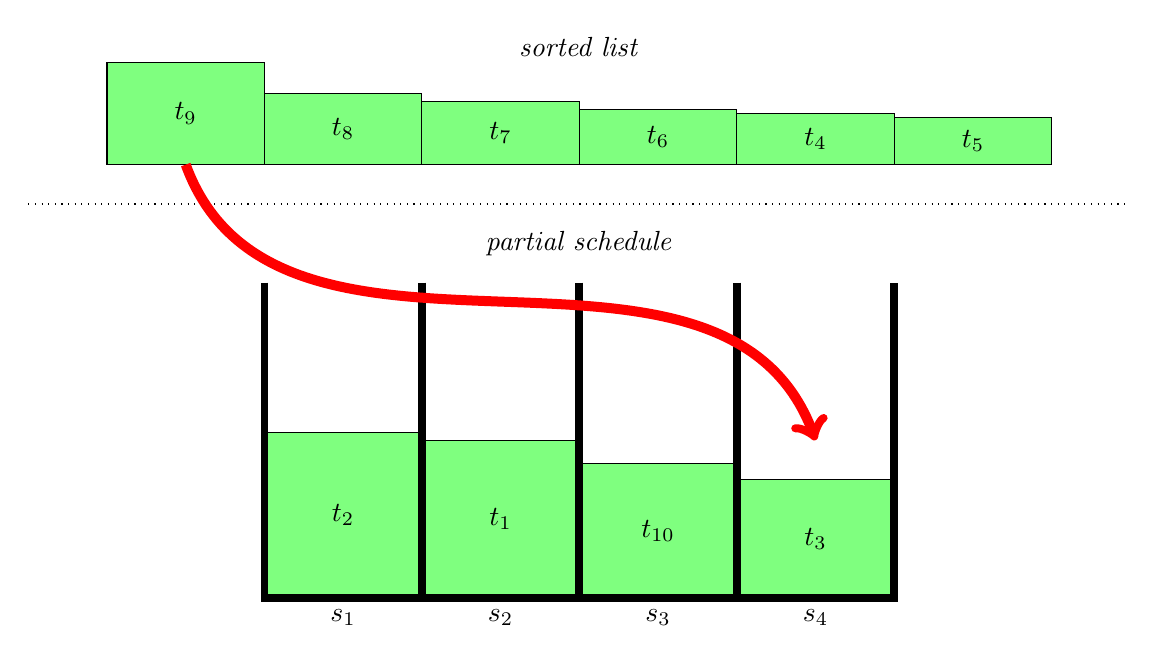
\begin{tikzpicture}
\definecolor{hlearn_bgbox}{RGB}{127,255,127}
\node[shape=rectangle,draw,fill=hlearn_bgbox,minimum width=2cm,minimum height=2.1cm] at (3,1.05) { $t_{2}$ };
\node[shape=rectangle,draw,fill=hlearn_bgbox,minimum width=2cm,minimum height=2.0cm] at (5,1) { $t_{1}$ };
\node[shape=rectangle,draw,fill=hlearn_bgbox,minimum width=2cm,minimum height=1.7cm] at (7,0.85) { $t_{10}$ };
\node[shape=rectangle,draw,fill=hlearn_bgbox,minimum width=2cm,minimum height=1.5cm] at (9,0.75) { $t_{3}$ };

\node[shape=rectangle,draw,fill=hlearn_bgbox,minimum width=2cm,minimum height=1.3cm] at (1,0.5+5.65) { $t_{9}$ };
\node[shape=rectangle,draw,fill=hlearn_bgbox,minimum width=2cm,minimum height=0.9cm] at (3,0.5+5.45) { $t_{8}$ };
\node[shape=rectangle,draw,fill=hlearn_bgbox,minimum width=2cm,minimum height=0.8cm] at (5,0.5+5.4) { $t_{7}$ };
\node[shape=rectangle,draw,fill=hlearn_bgbox,minimum width=2cm,minimum height=0.7cm] at (7,0.5+5.35) { $t_{6}$ };
\node[shape=rectangle,draw,fill=hlearn_bgbox,minimum width=2cm,minimum height=0.65cm] at (9,0.5+5.325) { $t_{4}$ };
\node[shape=rectangle,draw,fill=hlearn_bgbox,minimum width=2cm,minimum height=0.6cm] at (11,0.5+5.3) { $t_{5}$ };

\node at (6,4.5) {\emph{partial schedule}};
\node at (6,7) {\emph{sorted list}};
\draw[dotted] (-1,5) to (13,5);

\draw[line width=0.1cm] (2,4) to (2,0) to (2+2,0) to (2+2,4);
\draw[line width=0.1cm] (4,4) to (4,0) to (4+2,0) to (4+2,4);
\draw[line width=0.1cm] (6,4) to (6,0) to (6+2,0) to (6+2,4);
\draw[line width=0.1cm] (8,4) to (8,0) to (8+2,0) to (8+2,4);

\draw[->,line width=0.05in,color=red] (1,5.5) to [in=110,out=-70] (9,2);

\node at (3,-0.25) {$s_1$};
\node at (5,-0.25) {$s_2$};
\node at (7,-0.25) {$s_3$};
\node at (9,-0.25) {$s_4$};
\end{tikzpicture}
\vspace{0.1in}
\end{figure}

In HLearn, this conversion process is implemented with the internal function \lstinline{lptf}, as shown in Figure \ref{code:lptf} below.
The details of this function aren't particularly important.
What is important is that \lstinline{lptf} runs in time $\Theta(n\log p)$.

\begin{figure}
\caption{An implementation of the LPTF algorithm}
\label{code:lptf}
\begin{lstlisting}
lptf :: (Norm a) => Int -> SortedVector a -> Map.Map Int [a]
lptf p vector = snd $ F.foldr cata (emptyheap p,Map.empty) vector
    where
        emptyheap p = Heap.fromAscList [(0,i) | i<-[1..p]]
        cata x (heap,map) = 
            let Just top = Heap.viewHead heap
                set = snd top
                prio = (fst top)+magnitude x
                heap' = Heap.insert (prio,set) (Heap.drop 1 heap)
                map' = Map.insertWith (++) set [x] map
            in (heap',map')

\end{lstlisting}
\end{figure}

Now, the question remains, how are we going to define our monoid instance for \lstinline{Scheduling}?

\begin{lstlisting}
vector2scheduling :: forall a n. (Norm a, SingI n) => SortedVector a -> Scheduling n a
vector2scheduling vector = Scheduling
    { vector = vector
    , schedule = lptf (fromIntegral $ fromSing (sing :: Sing n)) vector
    }
\end{lstlisting}

Now, we can use this helper to define Monoid and homTrainer instances.

\begin{lstlisting}
instance (Ord a, Norm a, SingI n) => Monoid (Scheduling n a) where
    mempty = vector2scheduling mempty
    p1 `mappend` p2 = vector2scheduling $ (vector p1) <> (vector p2)

instance (Ord a, Norm a, SingI n) => HomTrainer (Scheduling n a) where
    type Datapoint (Scheduling n a) = a
    train1dp dp = vector2scheduling $ train1dp dp
\end{lstlisting}

The monoid instance is illustrated in Figure \ref{fig:monoid-detail}.

\begin{figure}[H]
\caption{The Monoid operation in detail}
\label{fig:monoid-detail}
\centering
\begin{tikzpicture}
\node at (-2.5in,4) {
    \resizebox{2in}{!}{
    \begin{tikzpicture}
    \definecolor{hlearn_bgbox}{RGB}{127,255,127}
    \definecolor{hlearn_bgboxB}{RGB}{191,191,255}
    \node[shape=rectangle,draw,fill=hlearn_bgbox,minimum width=2cm,minimum height=3.1cm]   at (1,1.55) { $t_{a,3}$ };;
    \node[shape=rectangle,draw,fill=hlearn_bgbox,minimum width=2cm,minimum height=2.7cm]   at (3,1.35) { $t_{a,2}$ };
    \node[shape=rectangle,draw,fill=hlearn_bgbox,minimum width=2cm,minimum height=2.1cm]   at (5,1.05) { $t_{a,1}$ };
    \node[shape=rectangle,draw,fill=hlearn_bgbox,minimum width=2cm,minimum height=1.7cm]   at (7,0.85) { $t_{a,4}$ };
    \node[shape=rectangle,draw,fill=hlearn_bgbox,minimum width=2cm,minimum height=1.6cm]   at (9,0.8) { $t_{a,5}$ };
    \node[shape=rectangle,draw,fill=hlearn_bgbox,minimum width=2cm,minimum height=0.6cm]   at (11,0.3) { $t_{a,6}$ };
    \end{tikzpicture}
    }};

\node at (-2.5in,0) {
    \resizebox{1.5in}{!}{
    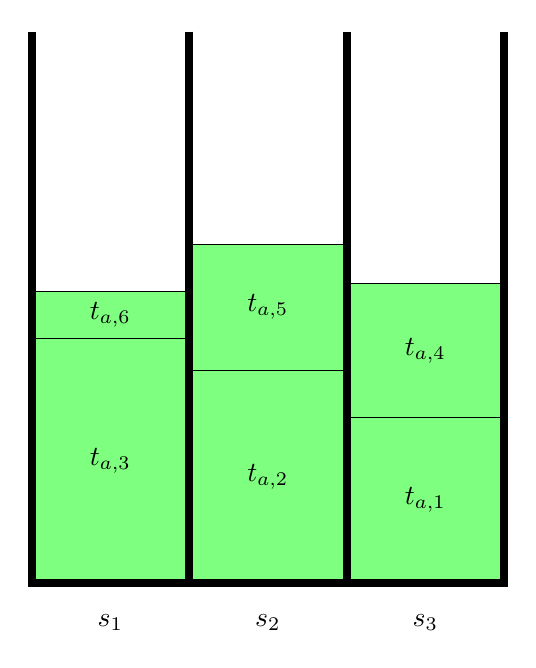
\begin{tikzpicture}
    \definecolor{hlearn_bgbox}{RGB}{127,255,127}
    \node[shape=rectangle,draw,fill=hlearn_bgbox,minimum width=2cm,minimum height=3.1cm] at (3,1.55) { $t_{a,3}$ };
    \node[shape=rectangle,draw,fill=hlearn_bgbox,minimum width=2cm,minimum height=0.6cm] at (3,3.4) { $t_{a,6}$ };
    \node[shape=rectangle,draw,fill=hlearn_bgbox,minimum width=2cm,minimum height=2.7cm] at (5,1.35) { $t_{a,2}$ };
    \node[shape=rectangle,draw,fill=hlearn_bgbox,minimum width=2cm,minimum height=1.6cm] at (5,3.5) { $t_{a,5}$ };
    \node[shape=rectangle,draw,fill=hlearn_bgbox,minimum width=2cm,minimum height=2.1cm] at (7,1.05) { $t_{a,1}$ };
    \node[shape=rectangle,draw,fill=hlearn_bgbox,minimum width=2cm,minimum height=1.7cm] at (7,2.95) { $t_{a,4}$ };
    \draw[line width=0.1cm] (2,7.0) to (2,0) to (2+2,0) to (2+2,7.0);
    \draw[line width=0.1cm] (4,7.0) to (4,0) to (4+2,0) to (4+2,7.0);
    \draw[line width=0.1cm] (6,7.0) to (6,0) to (6+2,0) to (6+2,7.0);
    \node at (3,-0.5) {$s_{1}$};
    \node at (5,-0.5) {$s_{2}$};
    \node at (7,-0.5) {$s_{3}$};
    \end{tikzpicture}
    }};

\node at (0.5,4) {
    \resizebox{2in}{!}{
    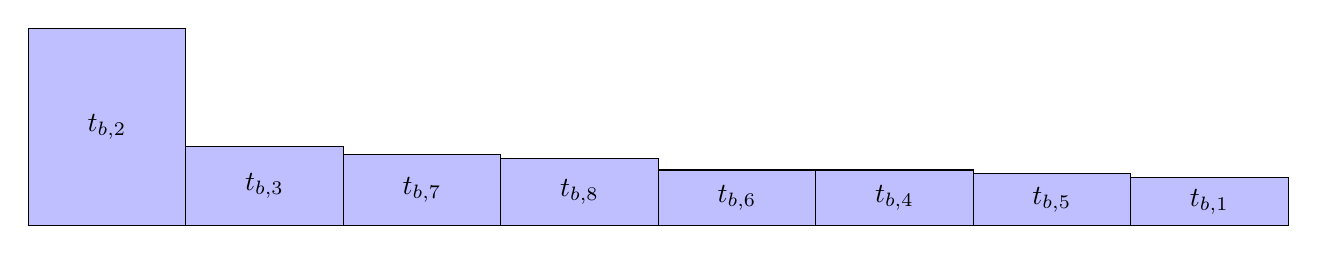
\begin{tikzpicture}
    \definecolor{hlearn_bgbox}{RGB}{127,255,127}
    \definecolor{hlearn_bgboxB}{RGB}{191,191,255}
    \node[shape=rectangle,draw,fill=hlearn_bgboxB,minimum width=2cm,minimum height=2.5cm]  at (1,1.25) { $t_{b,2}$ };
    \node[shape=rectangle,draw,fill=hlearn_bgboxB,minimum width=2cm,minimum height=1.0cm]  at (3,0.5) { $t_{b,3}$ };
    \node[shape=rectangle,draw,fill=hlearn_bgboxB,minimum width=2cm,minimum height=0.9cm]  at (5,0.45) { $t_{b,7}$ };
    \node[shape=rectangle,draw,fill=hlearn_bgboxB,minimum width=2cm,minimum height=0.85cm] at (7,0.425) { $t_{b,8}$ };
    \node[shape=rectangle,draw,fill=hlearn_bgboxB,minimum width=2cm,minimum height=0.7cm]  at (9,0.35) { $t_{b,6}$ };
    \node[shape=rectangle,draw,fill=hlearn_bgboxB,minimum width=2cm,minimum height=0.7cm]  at (11,0.35) { $t_{b,4}$ };
    \node[shape=rectangle,draw,fill=hlearn_bgboxB,minimum width=2cm,minimum height=0.65cm] at (13,0.325) { $t_{b,5}$ };
    \node[shape=rectangle,draw,fill=hlearn_bgboxB,minimum width=2cm,minimum height=0.6cm]  at (15,0.3) { $t_{b,1}$ };
    \end{tikzpicture}
    }};

\node at (0.5,0) {
    \resizebox{1.5in}{!}{
    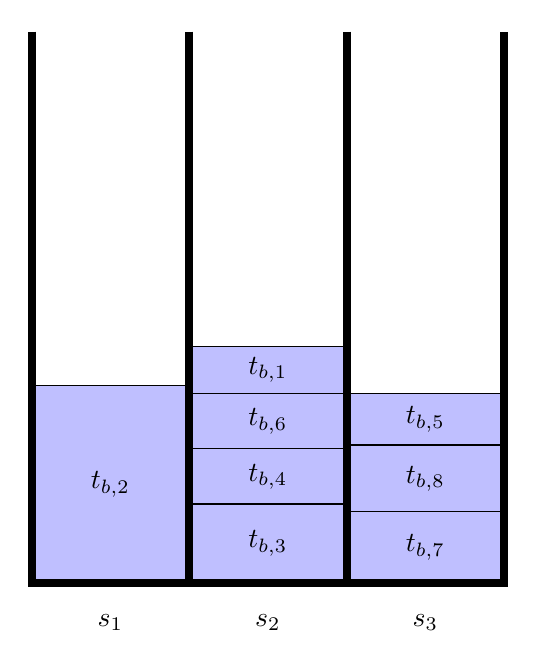
\begin{tikzpicture}
    \definecolor{hlearn_bgboxB}{RGB}{191,191,255}
    \node[shape=rectangle,draw,fill=hlearn_bgboxB,minimum width=2cm,minimum height=2.5cm] at (3,1.25) { $t_{b,2}$ };
    \node[shape=rectangle,draw,fill=hlearn_bgboxB,minimum width=2cm,minimum height=1.0cm] at (5,0.5) { $t_{b,3}$ };
    \node[shape=rectangle,draw,fill=hlearn_bgboxB,minimum width=2cm,minimum height=0.7cm] at (5,1.35) { $t_{b,4}$ };
    \node[shape=rectangle,draw,fill=hlearn_bgboxB,minimum width=2cm,minimum height=0.7cm] at (5,2.05) { $t_{b,6}$ };
    \node[shape=rectangle,draw,fill=hlearn_bgboxB,minimum width=2cm,minimum height=0.6cm] at (5,2.6999999999999997) { $t_{b,1}$ };
    \node[shape=rectangle,draw,fill=hlearn_bgboxB,minimum width=2cm,minimum height=0.9cm] at (7,0.45) { $t_{b,7}$ };
    \node[shape=rectangle,draw,fill=hlearn_bgboxB,minimum width=2cm,minimum height=0.85cm] at (7,1.325) { $t_{b,8}$ };
    \node[shape=rectangle,draw,fill=hlearn_bgboxB,minimum width=2cm,minimum height=0.65cm] at (7,2.075) { $t_{b,5}$ };
    \draw[line width=0.1cm] (2,7.0) to (2,0) to (2+2,0) to (2+2,7.0);
    \draw[line width=0.1cm] (4,7.0) to (4,0) to (4+2,0) to (4+2,7.0);
    \draw[line width=0.1cm] (6,7.0) to (6,0) to (6+2,0) to (6+2,7.0);
    \node at (3,-0.5) {$s_{1}$};
    \node at (5,-0.5) {$s_{2}$};
    \node at (7,-0.5) {$s_{3}$};
    \end{tikzpicture}
    }};

\node at (-1in,-4) {
    \resizebox{5in}{!}{
    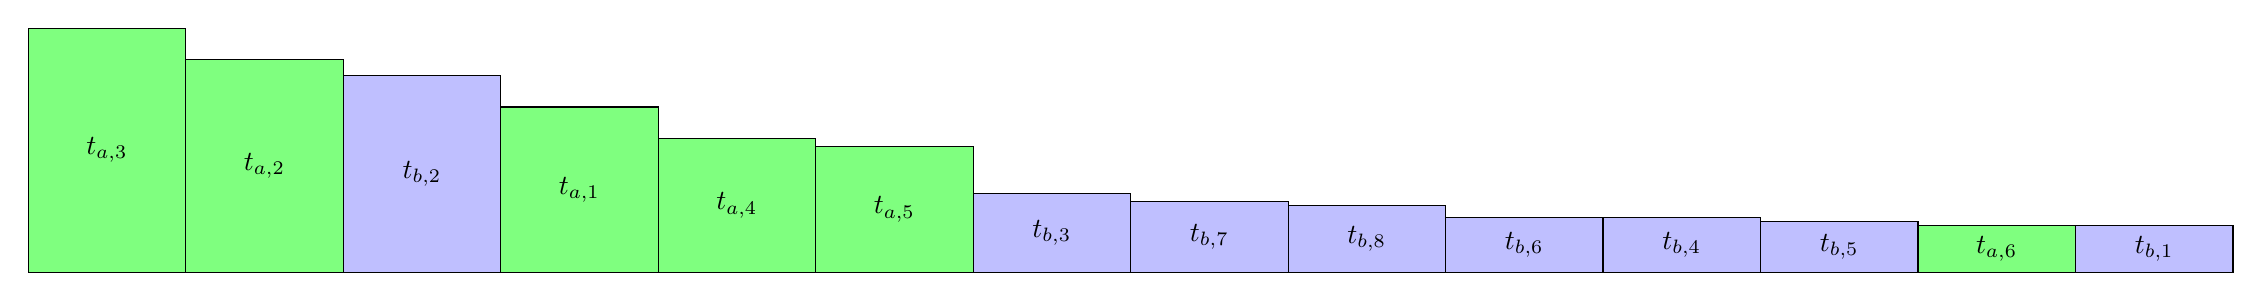
\begin{tikzpicture}
    \definecolor{hlearn_bgbox}{RGB}{127,255,127}
    \definecolor{hlearn_bgboxB}{RGB}{191,191,255}
    \node[shape=rectangle,draw,fill=hlearn_bgbox,minimum width=2cm,minimum height=3.1cm]   at (1,1.55) { $t_{a,3}$ };;
    \node[shape=rectangle,draw,fill=hlearn_bgbox,minimum width=2cm,minimum height=2.7cm]   at (3,1.35) { $t_{a,2}$ };
    \node[shape=rectangle,draw,fill=hlearn_bgboxB,minimum width=2cm,minimum height=2.5cm]  at (5,1.25) { $t_{b,2}$ };
    \node[shape=rectangle,draw,fill=hlearn_bgbox,minimum width=2cm,minimum height=2.1cm]   at (7,1.05) { $t_{a,1}$ };
    \node[shape=rectangle,draw,fill=hlearn_bgbox,minimum width=2cm,minimum height=1.7cm]   at (9,0.85) { $t_{a,4}$ };
    \node[shape=rectangle,draw,fill=hlearn_bgbox,minimum width=2cm,minimum height=1.6cm]   at (11,0.8) { $t_{a,5}$ };
    \node[shape=rectangle,draw,fill=hlearn_bgboxB,minimum width=2cm,minimum height=1.0cm]  at (13,0.5) { $t_{b,3}$ };
    \node[shape=rectangle,draw,fill=hlearn_bgboxB,minimum width=2cm,minimum height=0.9cm]  at (15,0.45) { $t_{b,7}$ };
    \node[shape=rectangle,draw,fill=hlearn_bgboxB,minimum width=2cm,minimum height=0.85cm] at (17,0.425) { $t_{b,8}$ };
    \node[shape=rectangle,draw,fill=hlearn_bgboxB,minimum width=2cm,minimum height=0.7cm]  at (19,0.35) { $t_{b,6}$ };
    \node[shape=rectangle,draw,fill=hlearn_bgboxB,minimum width=2cm,minimum height=0.7cm]  at (21,0.35) { $t_{b,4}$ };
    \node[shape=rectangle,draw,fill=hlearn_bgboxB,minimum width=2cm,minimum height=0.65cm] at (23,0.325) { $t_{b,5}$ };
    \node[shape=rectangle,draw,fill=hlearn_bgbox,minimum width=2cm,minimum height=0.6cm]   at (25,0.3) { $t_{a,6}$ };
    \node[shape=rectangle,draw,fill=hlearn_bgboxB,minimum width=2cm,minimum height=0.6cm]  at (27,0.3) { $t_{b,1}$ };
    \end{tikzpicture}
    }};
    
\node at (-1in,-8) {
    \resizebox{1.5in}{!}{
    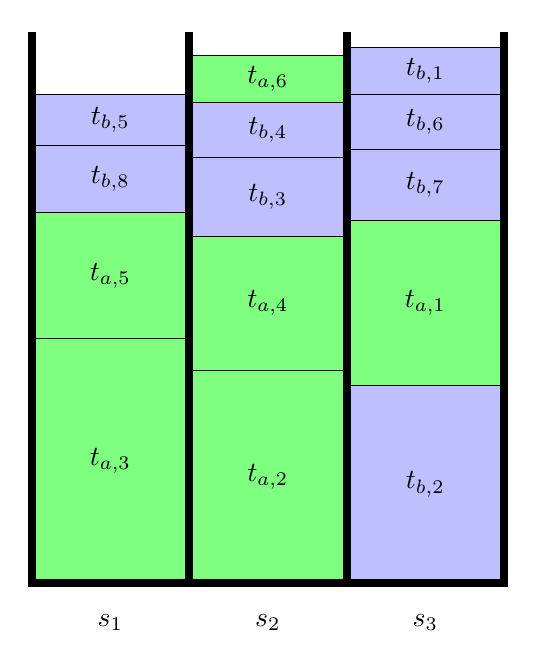
\begin{tikzpicture}
    \definecolor{hlearn_bgbox}{RGB}{127,255,127}
    \definecolor{hlearn_bgboxB}{RGB}{191,191,255}
    \node[shape=rectangle,draw,fill=hlearn_bgbox,minimum width=2cm,minimum height=3.1cm] at (3,1.55) { $t_{a,3}$ };
    \node[shape=rectangle,draw,fill=hlearn_bgbox,minimum width=2cm,minimum height=1.6cm] at (3,3.9000000000000004) { $t_{a,5}$ };
    \node[shape=rectangle,draw,fill=hlearn_bgboxB,minimum width=2cm,minimum height=0.85cm] at (3,5.125) { $t_{b,8}$ };
    \node[shape=rectangle,draw,fill=hlearn_bgboxB,minimum width=2cm,minimum height=0.65cm] at (3,5.875) { $t_{b,5}$ };
    \node[shape=rectangle,draw,fill=hlearn_bgbox,minimum width=2cm,minimum height=2.7cm] at (5,1.35) { $t_{a,2}$ };
    \node[shape=rectangle,draw,fill=hlearn_bgbox,minimum width=2cm,minimum height=1.7cm] at (5,3.5500000000000003) { $t_{a,4}$ };
    \node[shape=rectangle,draw,fill=hlearn_bgboxB,minimum width=2cm,minimum height=1.0cm] at (5,4.9) { $t_{b,3}$ };
    \node[shape=rectangle,draw,fill=hlearn_bgboxB,minimum width=2cm,minimum height=0.7cm] at (5,5.75) { $t_{b,4}$ };
    \node[shape=rectangle,draw,fill=hlearn_bgbox,minimum width=2cm,minimum height=0.6cm] at (5,6.4) { $t_{a,6}$ };
    \node[shape=rectangle,draw,fill=hlearn_bgboxB,minimum width=2cm,minimum height=2.5cm] at (7,1.25) { $t_{b,2}$ };
    \node[shape=rectangle,draw,fill=hlearn_bgbox,minimum width=2cm,minimum height=2.1cm] at (7,3.55) { $t_{a,1}$ };
    \node[shape=rectangle,draw,fill=hlearn_bgboxB,minimum width=2cm,minimum height=0.9cm] at (7,5.05) { $t_{b,7}$ };
    \node[shape=rectangle,draw,fill=hlearn_bgboxB,minimum width=2cm,minimum height=0.7cm] at (7,5.85) { $t_{b,6}$ };
    \node[shape=rectangle,draw,fill=hlearn_bgboxB,minimum width=2cm,minimum height=0.6cm] at (7,6.5) { $t_{b,1}$ };
    \draw[line width=0.1cm] (2,7.0) to (2,0) to (2+2,0) to (2+2,7.0);
    \draw[line width=0.1cm] (4,7.0) to (4,0) to (4+2,0) to (4+2,7.0);
    \draw[line width=0.1cm] (6,7.0) to (6,0) to (6+2,0) to (6+2,7.0);
    \node at (3,-0.5) {$s_{1}$};
    \node at (5,-0.5) {$s_{2}$};
    \node at (7,-0.5) {$s_{3}$};
    \end{tikzpicture}
    }};

\node at (-1in,0) {$\diamond$};

\draw[dotted] (-3.8in,-3) to (1.8in,-3);

\end{tikzpicture}
\end{figure}

So, we've argued that these instances are correct in the sense that they give us the right answers.
But what about our run times?

Well, the HomTrainer class provides a number of guarantees on that front.
In particular, if we know the run time of our monoid instance, then we can calculate the run time for sequential batch training, parallel batch training, and online training.
These results are shown in Table \ref{table:rt} below.

\begin{table}[H]
\caption{Run time guarantees for HomTrainer instances}
\label{table:rt}
\centering
\begin{tabular}{ c | c | c}
\hline
Monoid operation & Sequential batch trainer & \ \ Parallel batch trainer\ \ \\
\hline \hline
$O(1)$ & $O(n)$ & $O\left(\frac{n}{p}+\log p\right)$\\
$O(\log^a n)$, $a>0$ & $O(n)$ & $O\left(\frac{n}{p}+(\log^a n)(\log p)\right)$\\
$O(n)$ & $O(n\log n)$ & $O\left(\frac{n}{p}\log\frac{n}{p}+n\right)$\\
$O(n^b)$, $b>1$ & $O(n^b)$ & no improvement\\
\hline
\end{tabular}
\end{table}

In our case, we know that our monoid operation takes time $\Theta(n)$, and so our sequential batch trainer takes time $\Theta(n\log n)$.
Awesome!
That's exactly how long the LPTF algorithm is supposed to take.

Notice that BST is declared strict, whereas sets is declared lazy.

\section{Back to \prob{Bin Packing}}

We can deriving a Bin Packing instance similarly to how we derived a Scheduling instance.
We'll use an algorithn called Best Fit Decreasing (BFD).
$$
BFD \le {11\over9}OPT + 1
$$
And like LPTF, BFD takes time $\Theta(n\log n)$.
The dominating time is sorting a vector of the input elements.

\begin{figure}[H]
\caption{The Best First Decreasing (BFD) algorithm}
\label{fig:binpacking}
\centering
\begin{tikzpicture}

\node at (0,4) {
    \resizebox{3in}{!}{
    \begin{tikzpicture}
    \definecolor{hlearn_bgbox}{RGB}{127,255,127}
    \node[shape=rectangle,draw,fill=hlearn_bgbox,minimum width=2cm,minimum height=2.1cm] at (1,1.05) { $t_{2}$ };
    \node[shape=rectangle,draw,fill=hlearn_bgbox,minimum width=2cm,minimum height=2.0cm] at (3,1.0) { $t_{1}$ };
    \node[shape=rectangle,draw,fill=hlearn_bgbox,minimum width=2cm,minimum height=1.7cm] at (5,0.85) { $t_{10}$ };
    \node[shape=rectangle,draw,fill=hlearn_bgbox,minimum width=2cm,minimum height=1.5cm] at (7,0.75) { $t_{3}$ };
    \node[shape=rectangle,draw,fill=hlearn_bgbox,minimum width=2cm,minimum height=1.3cm] at (9,0.65) { $t_{9}$ };
    \node[shape=rectangle,draw,fill=hlearn_bgbox,minimum width=2cm,minimum height=0.9cm] at (11,0.45) { $t_{8}$ };
    \node[shape=rectangle,draw,fill=hlearn_bgbox,minimum width=2cm,minimum height=0.8cm] at (13,0.4) { $t_{7}$ };
    \node[shape=rectangle,draw,fill=hlearn_bgbox,minimum width=2cm,minimum height=0.7cm] at (15,0.35) { $t_{6}$ };
    \node[shape=rectangle,draw,fill=hlearn_bgbox,minimum width=2cm,minimum height=0.65cm] at (17,0.325) { $t_{4}$ };
    \node[shape=rectangle,draw,fill=hlearn_bgbox,minimum width=2cm,minimum height=0.6cm] at (19,0.3) { $t_{5}$ };
    \end{tikzpicture}
    }};

\node at (0,0) {
    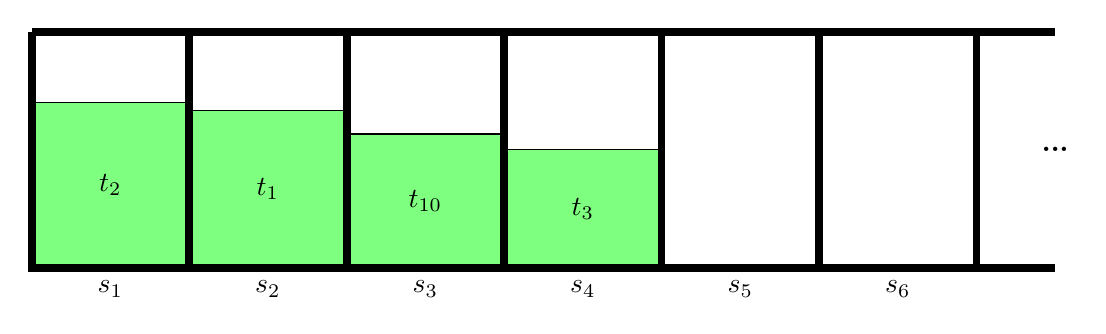
\begin{tikzpicture}
    \definecolor{hlearn_bgbox}{RGB}{127,255,127}
    \node[shape=rectangle,draw,fill=hlearn_bgbox,minimum width=2cm,minimum height=2.1cm] at (3,1.05) { $t_{2}$ };
%     \node[shape=rectangle,draw,fill=hlearn_bgbox,minimum width=2cm,minimum height=0.7cm] at (3,2.45) { $t_{6}$ };
    \node[shape=rectangle,draw,fill=hlearn_bgbox,minimum width=2cm,minimum height=2.0cm] at (5,1.0) { $t_{1}$ };
%     \node[shape=rectangle,draw,fill=hlearn_bgbox,minimum width=2cm,minimum height=0.8cm] at (5,2.4) { $t_{7}$ };
    \node[shape=rectangle,draw,fill=hlearn_bgbox,minimum width=2cm,minimum height=1.7cm] at (7,0.85) { $t_{10}$ };
%     \node[shape=rectangle,draw,fill=hlearn_bgbox,minimum width=2cm,minimum height=0.9cm] at (7,2.15) { $t_{8}$ };
    \node[shape=rectangle,draw,fill=hlearn_bgbox,minimum width=2cm,minimum height=1.5cm] at (9,0.75) { $t_{3}$ };
%     \node[shape=rectangle,draw,fill=hlearn_bgbox,minimum width=2cm,minimum height=1.3cm] at (9,2.15) { $t_{9}$ };
%     \node[shape=rectangle,draw,fill=hlearn_bgbox,minimum width=2cm,minimum height=0.65cm] at (11,0.325) { $t_{4}$ };
%     \node[shape=rectangle,draw,fill=hlearn_bgbox,minimum width=2cm,minimum height=0.6cm] at (11,0.95) { $t_{5}$ };
    \draw[line width=0.1cm] (2,3.0) to (2,0) to node[below] {$s_{1}$} (2+2,0) to (2+2,3.0);
    \draw[line width=0.1cm] (4,3.0) to (4,0) to node[below] {$s_{2}$} (4+2,0) to (4+2,3.0);
    \draw[line width=0.1cm] (6,3.0) to (6,0) to node[below] {$s_{3}$} (6+2,0) to (6+2,3.0);
    \draw[line width=0.1cm] (8,3.0) to (8,0) to node[below] {$s_{4}$} (8+2,0) to (8+2,3.0);
    \draw[line width=0.1cm] (10,3.0) to (10,0) to node[below] {$s_{5}$} (10+2,0) to (10+2,3.0);
    \draw[line width=0.1cm] (12,3.0) to (12,0) to node[below] {$s_{6}$} (12+2,0) to (12+2,3.0);
    % \draw[line width=0.1cm] (14,3.0) to (14,0) to node[below] {$s_{5}$} (14+2,0) to (14+2,3.0);
    % \draw[line width=0.1cm] (16,3.0) to (16,0) to node[below] {$s_{5}$} (16+2,0) to (16+2,3.0);
    \draw[line width=0.1cm] (2,3.0) to (15,3.0);
    \draw[line width=0.1cm] (2,0) to (15,0);
    % \draw[dashed,color=red,line width=0.05cm] (2,3) to (2,4);
    % \draw[dashed,color=red,line width=0.05cm] (12,3) to (12,4);
    % \draw[<->,line width=0.05cm,color=red] (2,3.5) to node[above] {number of bins} (12,3.5);
    % \draw[<->,line width=0.05cm,color=blue] (1.5,0) to (1.5,3);
    % \draw[dashed,color=blue,line width=0.05cm] (1,0) to (2,0);
    % \draw[dashed,color=blue,line width=0.05cm] (1,3) to (2,3);
    % \node[color=blue] at (1,1.5) {\rotatebox{90}{fixed bin size}};
    \node at (15,1.5) {\textbf{...}};
    \end{tikzpicture}
    };
    
\end{tikzpicture}
\end{figure}


\section{Takeaways}

I originally designed the HomTrainer type class for machine learning algorithms, but it's a lot more general than that.
It works on any functions that have type:
\begin{spec}
func :: [datapoint] -> m
\end{spec}
All you have to find a monoid instance for m.
Of course, this can be quite tricky.
In some cases, an appropriate monoid might not even exist.


\end{document}